The necropolis of Ramsey is a complex of underground mausoleums, buried by earth and time.
It is also where Dr. Jonas almost got fired. It seems that these mausoleums were cursed,
guaranteeing that the room containing hidden artifacts would always be as far away from her
excavation team as possible, wasting university resources.

To solve this problem, she made the following plan. To explore a masoleum, she would
send one or more research assistants into accessible rooms, each costing \$1000 in funds.
Then using advanced artifact-finding technology, she could pinpoint the location of the
hidden artifacts, and one of the closest assistants could then travel to that room 
(which is always as far away as possible, and might require traveling
through rooms inaccessible from the surface) and
extract the goods, costing another \$1000 per room explored.

I've attached an example of such a plan to this message. Each labeled circle
is a room of the masoleum accessible from the surface, and each gray circle
is inaccessible from the surface. There is a unique way to place assistants 
in the accessible rooms to minimize the total
cost of exploring this mausoleum to \$4000, which I've marked with squares.
 
I have a feeling that Dr. Jonas's February entry contains three of these
masoleum diagrams. Can you identify where to place assistants in each
to minimize the total cost of all three crypts?
Answer using ClueKeeper by listing all letters used in alphabetical order. -BF
\begin{center}
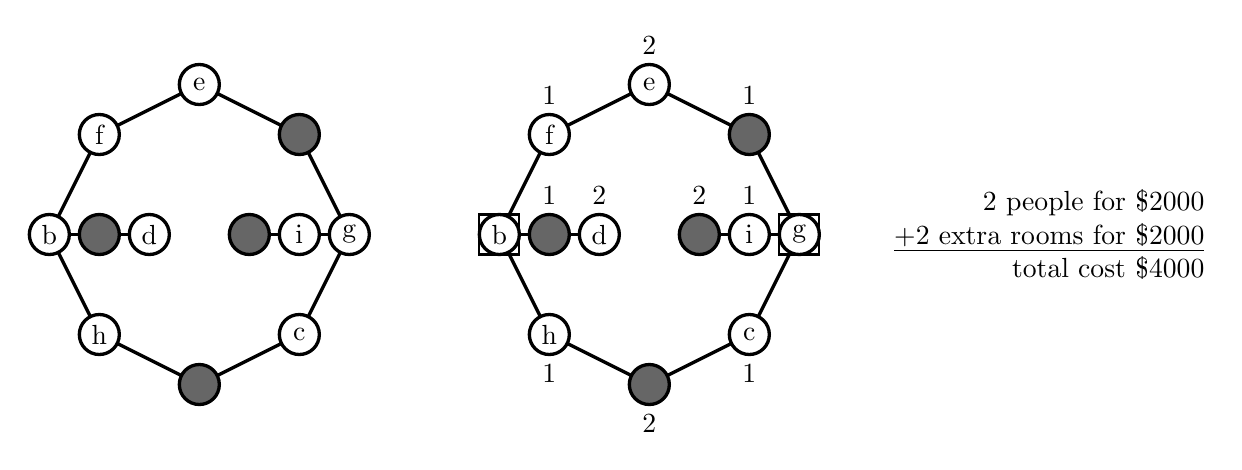
\begin{tikzpicture}[x=0.25in,y=0.25in]
    \draw [very thick] (-3,0) -- (-1,0);
    \draw [very thick] (3,0) -- (1,0);
    \draw [very thick] (-3,0) -- (-2,2) -- (0,3) -- (2,2) -- (3,0) -- (2,-2) -- (0,-3) -- (-2,-2) -- cycle;
    
    \draw [color = black, fill = white, very thick] (-3,0) circle (0.4);
      \node at (-3,0) {b};
    \draw [color = black, fill = black!60, very thick] (-2,0) circle (0.4);
    \draw [color = black, fill = white, very thick] (-1,0) circle (0.4);
      \node at (-1,0) {d};
    \draw [color = black, fill = white, very thick] (3,0) circle (0.4);
      \node at (3,0) {g};
    \draw [color = black, fill = white, very thick] (2,0) circle (0.4);
      \node at (2,0) {i};
    \draw [color = black, fill = black!60, very thick] (1,0) circle (0.4);
    \draw [color = black, fill = black!60, very thick] (0,-3) circle (0.4);
    \draw [color = black, fill = white, very thick] (0,3) circle (0.4);
      \node at (0,3) {e};
    \draw [color = black, fill = black!60, very thick] (2,2) circle (0.4);
    \draw [color = black, fill = white, very thick] (-2,2) circle (0.4);
      \node at (-2,2) {f};
    \draw [color = black, fill = white, very thick] (2,-2) circle (0.4);
      \node at (2,-2) {c};
    \draw [color = black, fill = white, very thick] (-2,-2) circle (0.4);
      \node at (-2,-2) {h};
\begin{scope}[shift={(9,0)}]
    \draw [very thick] (-3,0) -- (-1,0);
    \draw [very thick] (3,0) -- (1,0);
    \draw [very thick] (-3,0) -- (-2,2) -- (0,3) -- (2,2) -- (3,0) -- (2,-2) -- (0,-3) -- (-2,-2) -- cycle;
    
    \draw [color = black, fill = white, very thick] (-3,0) circle (0.4);
      \node at (-3,0) {b};
    \draw [color = black, fill = black!60, very thick] (-2,0) circle (0.4);
    \draw [color = black, fill = white, very thick] (-1,0) circle (0.4);
      \node at (-1,0) {d};
    \draw [color = black, fill = white, very thick] (3,0) circle (0.4);
      \node at (3,0) {g};
    \draw [color = black, fill = white, very thick] (2,0) circle (0.4);
      \node at (2,0) {i};
    \draw [color = black, fill = black!60, very thick] (1,0) circle (0.4);
    \draw [color = black, fill = black!60, very thick] (0,-3) circle (0.4);
    \draw [color = black, fill = white, very thick] (0,3) circle (0.4);
      \node at (0,3) {e};
    \draw [color = black, fill = black!60, very thick] (2,2) circle (0.4);
    \draw [color = black, fill = white, very thick] (-2,2) circle (0.4);
      \node at (-2,2) {f};
    \draw [color = black, fill = white, very thick] (2,-2) circle (0.4);
      \node at (2,-2) {c};
    \draw [color = black, fill = white, very thick] (-2,-2) circle (0.4);
      \node at (-2,-2) {h};

      \draw[thick] (-2.6,-0.4) -- (-2.6,0.4) -- (-3.4,0.4) -- (-3.4,-0.4) -- cycle;
      \draw[thick] (2.6,-0.4) -- (2.6,0.4) -- (3.4,0.4) -- (3.4,-0.4) -- cycle;
    \node[anchor=south] at (-1,0.4) {2};
    \node[anchor=south] at (-2,0.4) {1};
    \node[anchor=south] at (1,0.4) {2};
    \node[anchor=south] at (2,0.4) {1};
    \node[anchor=south] at (-2,2.4) {1};
    \node[anchor=south] at (2,2.4) {1};
    \node[anchor=north] at (-2,-2.4) {1};
    \node[anchor=north] at (2,-2.4) {1};
    \node[anchor=south] at (0,3.4) {2};
    \node[anchor=north] at (0,-3.4) {2};
\end{scope}
    \node[align=right] at (17,0) 
      {2 people for \$2000 \\ \underline{+2 extra rooms for \$2000} \\ total cost \$4000};
  \end{tikzpicture}
\end{center}
